\documentclass{beamer}
\usepackage[utf8]{inputenc}
\usepackage{listings}
\usepackage{hyperref}
\usepackage{graphicx}
%\usetheme{Darmstadt}

\title{An ARM backend for the stage2 zig compiler}
\author{Joachim Schmidt}
\date{10th October 2020}

\begin{document}

\frame{\titlepage}

\begin{frame}{@This()}
    \begin{itemize}
        \item<1-> Joachim Schmidt
        \item<2-> Technische Universität Darmstadt
        \item<3-> Fun fact about me: I like pizza
    \end{itemize}
\end{frame}

\begin{frame}{Overview}
    \tableofcontents
\end{frame}

\section{Compiler backends and stage2}

\begin{frame}{What is a compiler?}
\end{frame}

\begin{frame}{Compiling Hello World in zig}
\end{frame}

\begin{frame}{Where did the zig compiler come from?}
\end{frame}

\begin{frame}{Bootstrapping}
\end{frame}

\begin{frame}{The current plan}
\end{frame}

\begin{frame}{Backends}
\end{frame}

\section{ARM architecture}

\begin{frame}{von Neumann architecture}
\end{frame}

\begin{frame}[fragile]{CISC}
\begin{columns}
\column{0.4\textwidth}
\begin{verbatim}
export fn foo() u32 {
    var x: u32 = 42;
    var y: u32 = 23;
    return x + y;
}
\end{verbatim}

\column{0.6\textwidth}
\begin{verbatim}
...
mov     dword ptr [rbp - 8], 42
mov     dword ptr [rbp - 12], 23
mov     eax, dword ptr [rbp - 8]
add     eax, dword ptr [rbp - 12]
...
\end{verbatim}
\end{columns}

\vspace{1cm}

\url{https://zig.godbolt.org/z/qoMfEK}
\end{frame}

\begin{frame}[fragile]{RISC}
\begin{columns}
\column{0.4\textwidth}
\begin{verbatim}
export fn foo() u32 {
    var x: u32 = 42;
    var y: u32 = 23;
    return x + y;
}
\end{verbatim}

\column{0.6\textwidth}
\begin{verbatim}
...
movw    r0, #42
str     r0, [sp, #8]
movw    r0, #23
str     r0, [sp, #4]
ldr     r0, [sp, #8]
ldr     r1, [sp, #4]
adds    r0, r0, r1
...
\end{verbatim}
\end{columns}

\vspace{1cm}

\url{https://zig.godbolt.org/z/Mee9ro}
\end{frame}

\begin{frame}[fragile]{ARM instruction set}
\begin{itemize}
    \item<1-> Data Processing
    \begin{verbatim}
    add r0, r1, #2\end{verbatim}
    \item<2-> Memory
    \begin{verbatim}
    ldr r0, [sp, #4]\end{verbatim}
    \item<3-> Branching
    \begin{verbatim}
    b label
    bx lr\end{verbatim}
\end{itemize}
\end{frame}

\begin{frame}[fragile]{A brief look at the add instruction}
    \begin{verbatim}
    add r0, r1, #2\end{verbatim}
    \begin{figure}
        \centering
        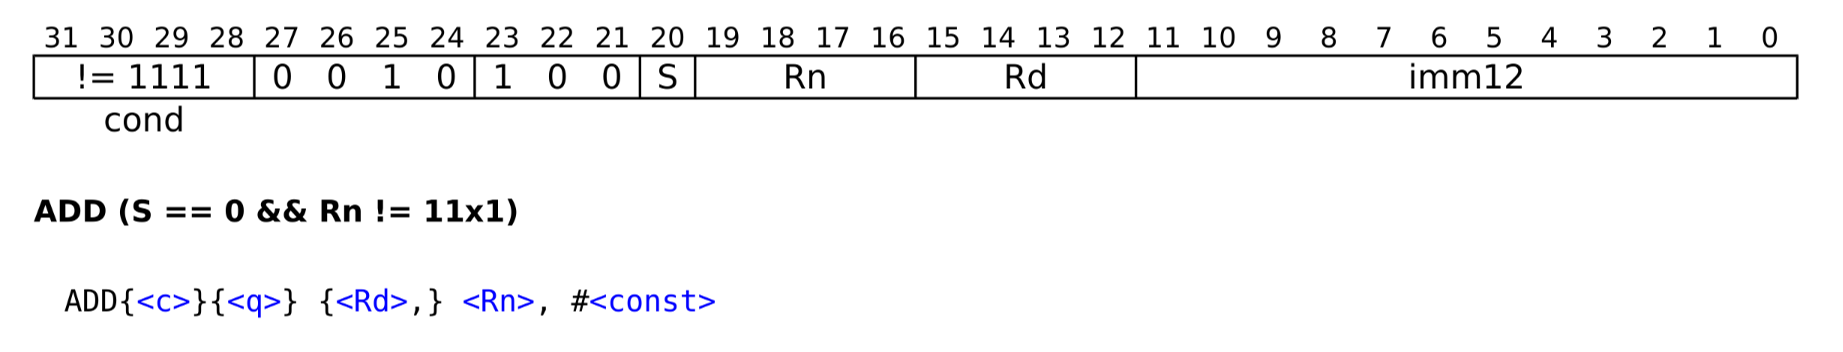
\includegraphics[width=\textwidth]{add.png}
        \caption{Encoding of add; Source: \cite{isa}}
        \label{fig:add}
    \end{figure}
\end{frame}

\begin{frame}[fragile]{Condition codes}
\begin{columns}
\column{0.6\textwidth}
\begin{verbatim}
export fn isAnswer(x: u32) u32 {
    return if (x == 42) 32
        else 12;
}
\end{verbatim}

\column{0.4\textwidth}
\begin{verbatim}
mov     r1, #12
cmp     r0, #42
movweq  r1, #32
mov     r0, r1
bx      lr
\end{verbatim}
\end{columns}

\vspace{1cm}

\url{https://zig.godbolt.org/z/q5rP8e}
\end{frame}

\section{Live demo on a Raspberry Pi}

\begin{frame}{Live demo}
    \begin{figure}
        \centering
        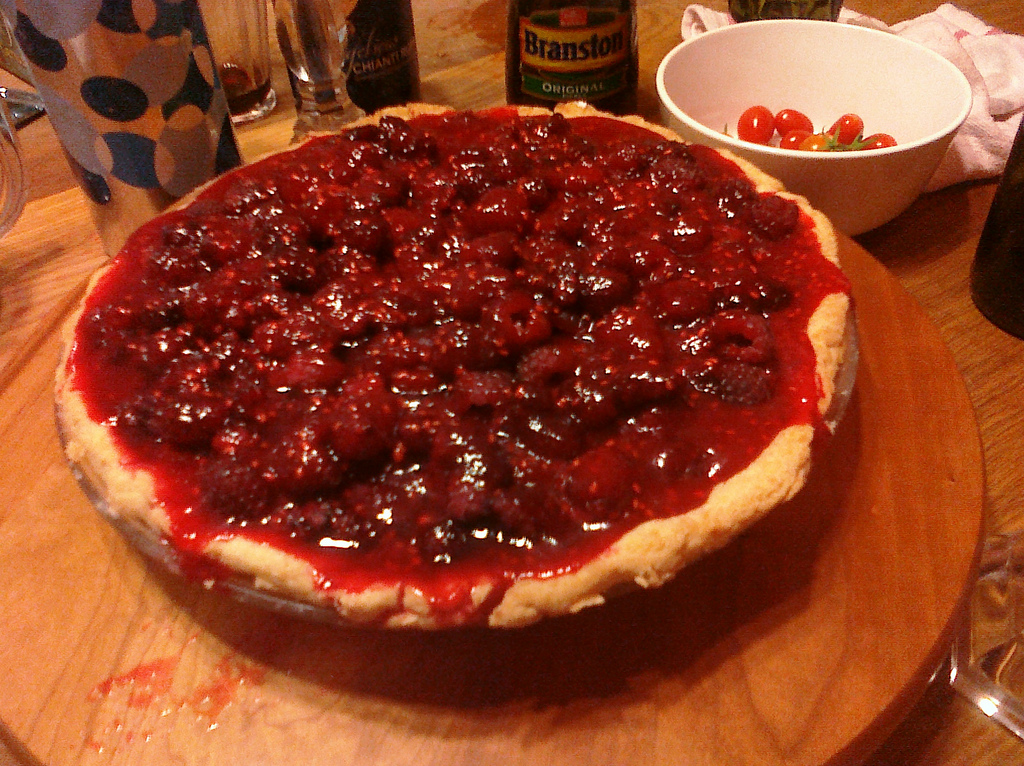
\includegraphics[width=0.8\textwidth]{Raspberry_pie.jpg}
        \caption{Source: \cite{rpie}}
        \label{fig:rpie}
    \end{figure}
\end{frame}

\section{Q \& A}

\begin{frame}{Q \& A}
    \begin{itemize}
        \item GitHub: \url{https://github.com/joachimschmidt557}
        \item Discord: \texttt{joachim.schmidt557\#6869}
        \item Matrix: \texttt{@joachimschmidt557:matrix.org}
    \end{itemize}
\end{frame}

\begin{frame}{References}
    \begin{thebibliography}{}
    \bibitem{rpie}
    \url{https://www.flickr.com/photos/rexroof/3802694376/}
    
    \bibitem{isa}
    \url{https://static.docs.arm.com/ddi0597/h/ISA_AArch32_xml_v86A-2020-06.pdf}
    
    \end{thebibliography}
\end{frame}

\end{document}
